% Figure 14 -- the Seiberg-Witten curve from the marked integer points
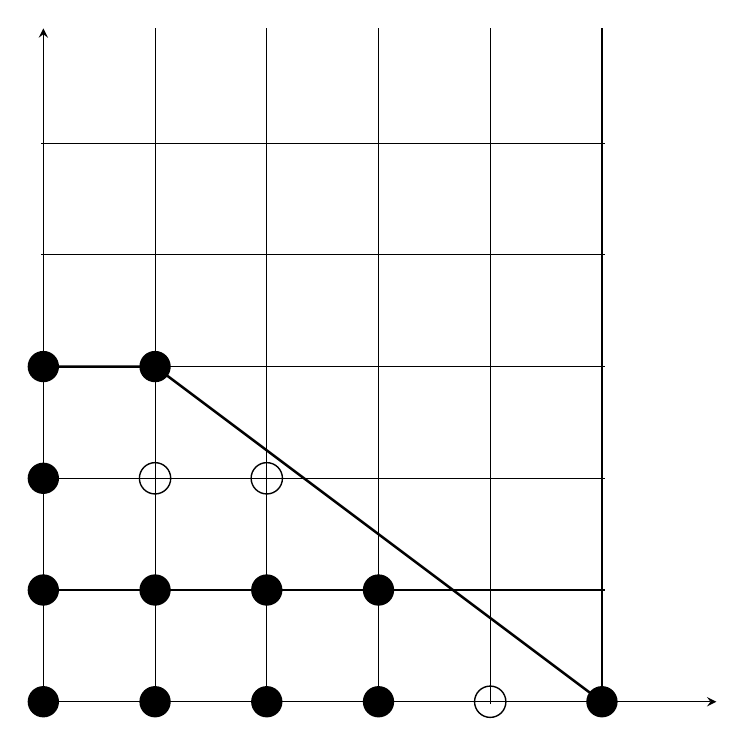
\begin{tikzpicture}[x=1pt,y=1pt,scale=1.08,transform shape,>=stealth,line width=0.5pt]
  \def\u{37.38}
  % ---- grid ----
  \foreach \i in {1,...,5} {\draw[line width=0.4pt] ({24.1+\i*\u},33.5) -- ({24.1+\i*\u},259.6);}
  \foreach \j in {1,...,5} {\draw[line width=0.4pt] (23.4,{34.3+\j*\u}) -- (211.96,{34.3+\j*\u});}
  % ---- axes ----
  \draw[->] (23.4,34.3) -- (249.3,34.3);
  \draw[->] (24.1,33.5) -- (24.1,259.6);
  % ---- Newton polygon ----
  \draw[line width=0.9pt] (24.1,{34.3+3*\u}) -- ({24.1+\u},{34.3+3*\u}) -- ({24.1+5*\u},34.3);
  % ---- marked lattice points ----
  \foreach \i/\j in {0/0,1/0,2/0,3/0,5/0,0/1,1/1,2/1,3/1,0/2,0/3,1/3}
    {\fill ({24.1+\i*\u},{34.3+\j*\u}) circle[radius=5.24pt];}
  \foreach \i/\j in {4/0,1/2,2/2}
    {\draw ({24.1+\i*\u},{34.3+\j*\u}) circle[radius=5.24pt];}
\end{tikzpicture}
